\begin{frame}[label=current]
\frametitle{Euclidean Distance in Coordinates}
\begin{definition}
The distance between the points $A(x_A,y_A,z_A)$ and $B(x_B,y_B,z_B)$ is given by:
\[
d(A,B) = |AB| = \sqrt{(x_B-x_A)^2+(y_B-y_A)^2+(z_B-z_A)^2}
\]
\end{definition}
\begin{columns}
\column{0.4\textwidth}
\psset{xunit=1cm, yunit=1cm}
\begin{pspicture}(-2, -2)(2,2)
\renewcommand{\fcScreen}{[-0.5 1 -0.2] -1}
\tiny
\fcAxesIIId{3}{3}{3}
\fcPolyLineIIId[linecolor=red]{[2.6 1 1][2.6 1.4 1] [3 1.4 1] }
\fcPolyLineIIId[linecolor=red]{[2.8 3.7 1][2.8 3.7 1.360555128] [3 4 1.360555128] }

\fcPolyLineIIId[linestyle=dotted]{ [1 1 1] [1 4 1] [1 4 3]}
\fcLineIIId[linestyle=dotted]{[1 4 1]}{[3 4 1]}
\fcParallelogramHollowIIId{ [1 1 1] }{ [3 1 1] }{ [3 1 3] }
\fcParallelogramHollowIIId{ [1 1 3] }{ [3 1 3] }{ [3 4 3] }
\fcParallelogramHollowIIId{ [3 1 1] }{ [3 4 1] }{ [3 4 3] }
\fcLineIIId[linestyle=dotted]{[1 1 1]}{[3 4 1]}
\fcLineIIId[linestyle=dotted]{[1 1 1]}{[3 4 3]}
\fcPutIIId[t]{[1 1 0.9]}{$A$}
\fcPutIIId[l]{[3 4 3]}{$~~B$}
\fcPutIIId[l]{[3 4 1]}{$~~C$}
\fcPutIIId[t]{[3 1 0.9]}{$D$}

\fcPutIIId[t]{[2 1 0.9]}{$x_B- x_A$}
\fcPutIIId[tl]{[3 2.5 1]}{$~~y_B- y_A$}

\fcPutIIId[l]{[3 4 2]}{$~~z_B- z_A$}
\end{pspicture}
\column{0.6\textwidth}
Motivation. 

Pythagorean theorem for $\triangle ADC$: $|AC|^2 = |AD|^2+|DC|^2$.
Pythagorean theorem for $\triangle ACB$: $|AB|^2 =|AC|^2+ |BC|^2= |AD|^2+|DC|^2+|BC|^2 = (x_B-x_A)^2+(y_B-y_A)^2+(z_B-z_A)^2$.
\end{columns}

%\psfrag{O}{$O$}
%\psfrag{A}{$A$} 
%\psfrag{B}{$B(x_B, y_B, z_B)$}  
%\psfrag{C}{$C(x_B, y_B, z_A)$}    
%\psfrag{x}{$y$} 
%\psfrag{y}{$x$} 
%\psfrag{z}{$z$}     
%\psfrag{dx}{$y_B - y_A$}
%\psfrag{dy}{$x_B - x_A$}
%\psfrag{dz}{$z_B - z_A$}  
%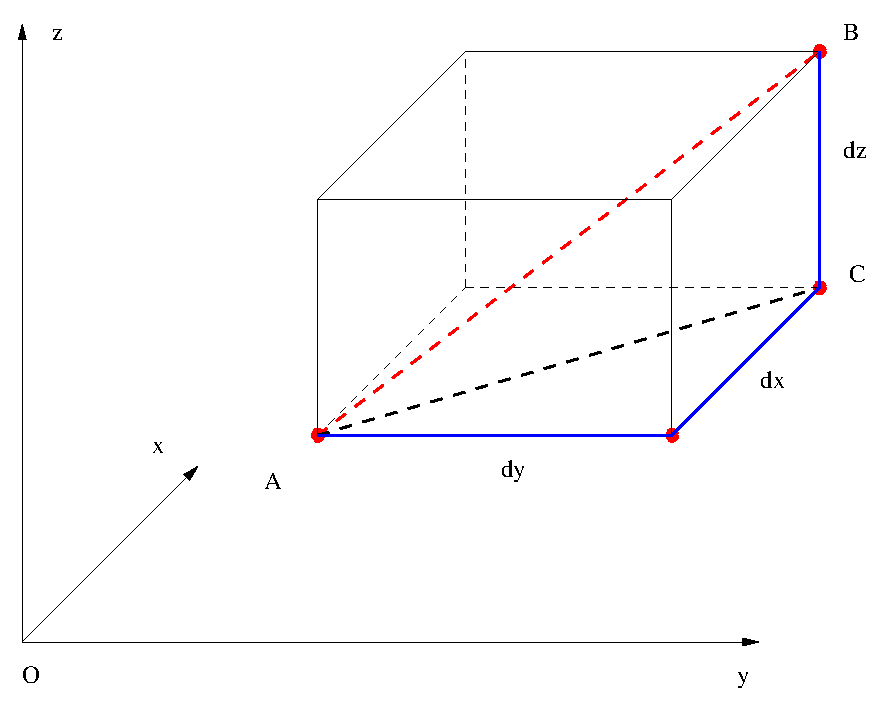
\includegraphics[height=1in]{../../modules/coordinate-systems/pictures/euclidean_distance.eps}
%
%
Example: $P(3,1,2)$ and $Q(1,2,3)$:\pause
%
$$D(P,Q) = \sqrt{(1-3)^2+(2-1)^2+(3-2)^2} = \sqrt{6}\; .$$

\end{frame}